% Chapter 6

\chapter{EVALUATION METRICS} % Write in your own chapter title
Off-the-hook-plus must be evaluated  for the following performance metrics, which become important as this is meant for users who will never need to know about computer programming. The metrics used here are as follows.

\begin{enumerate}
    \item Phish detection accuracy
    \item Target detection ratio
    \item Memory usage profiling
    \item Add-on rendering time
    \item Temporal resilience accuracy
\end{enumerate}

\section{PHISH DETECTION ACCURACY}
Phish detection accuracy is really important because the main task for this application is to notify the people if the site is a phish or not. It is defined as the ratio of the total number of correct classifications to the total number of classifications.\\
\null\quad\textit{Accuracy = (TP+TN)/(TP+TN+FP+FN)}\\

\begin{figure}[htp]
\centering
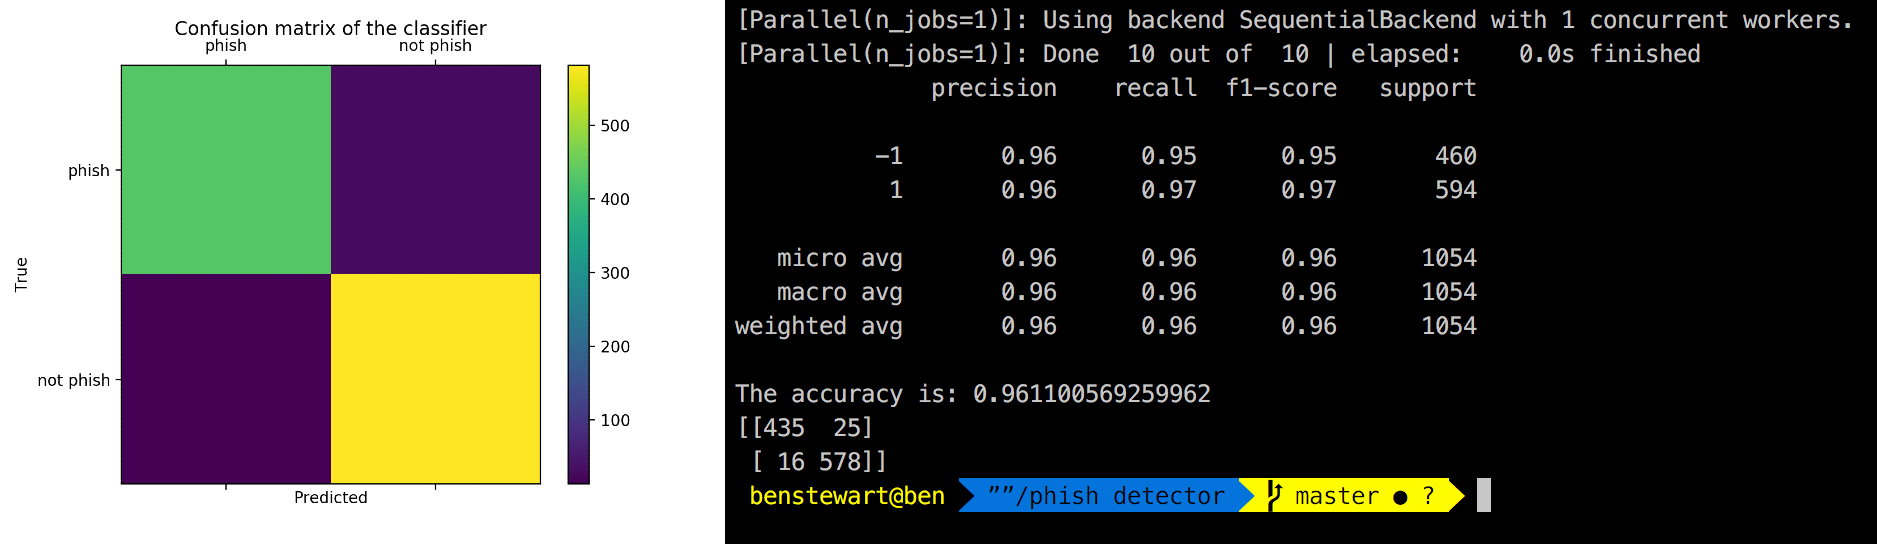
\includegraphics[scale=0.2]{Figures/image1.png}
\caption{Phish Detection Confusion Matrix and Metrics}
\label{fig:pdcmm}
\end{figure}

The Figure ~\ref{fig:pdcmm} gives the phish detection accuracy along with the precision, recall and f1-score. It also has the confusion matrix that gives a visual representation of how the model tags the web pages.

\section{TARGET DETECTION RATIO}
Target detection ratio is to measure the ease of use for the user by providing them with the original site which is being mimicked by the phish. This will be the ratio of phish sites whose target has been found to that of the total number of phish sites.\\
\null\quad\textit{Detection Ratio = (TP)/(TP+TN+FP+FN)}\\

\begin{figure}[htp]
\centering
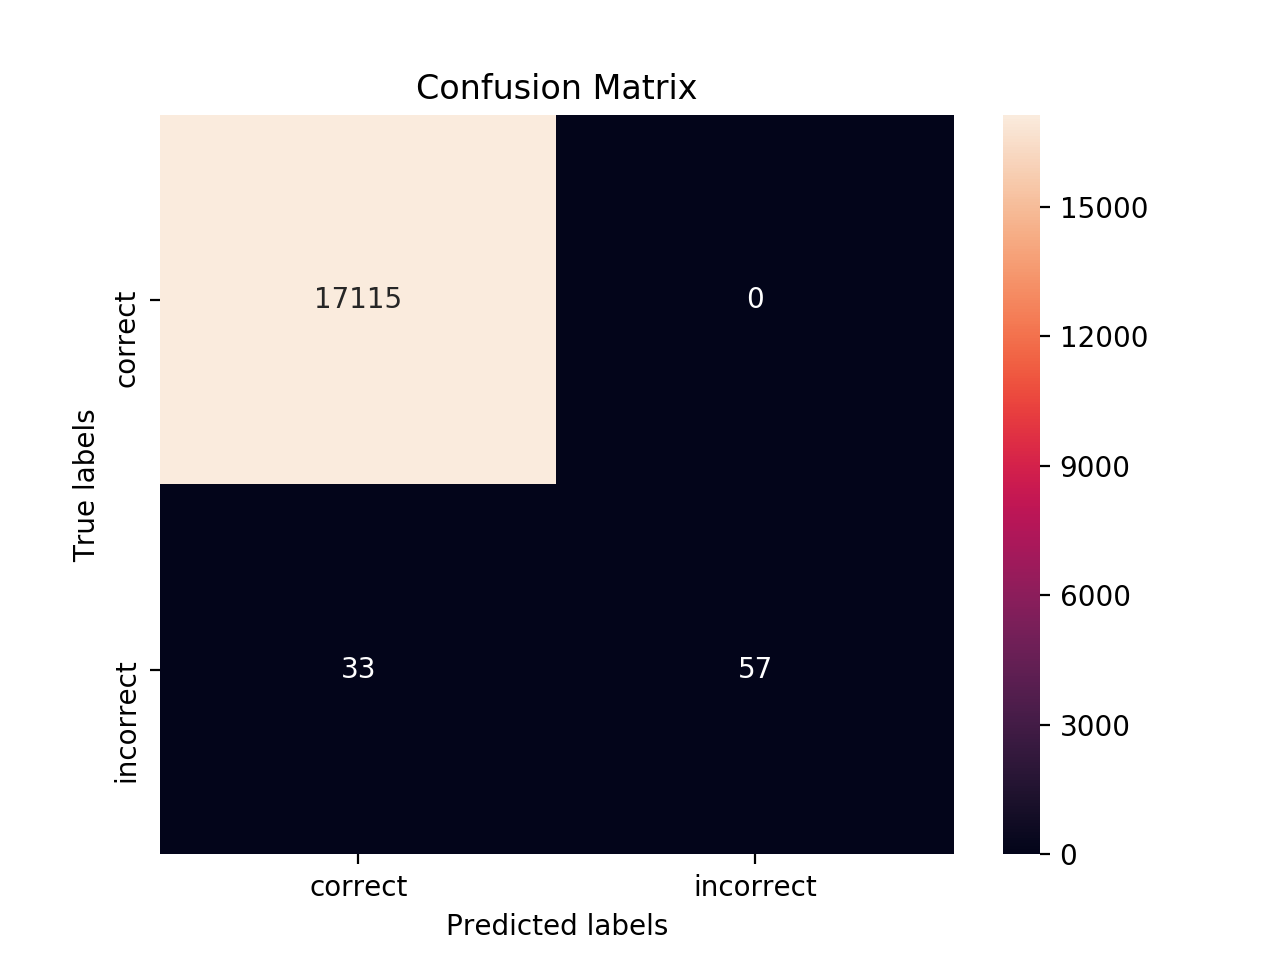
\includegraphics[scale=0.5]{Figures/image4.png}
\caption{Target Detection Confusion Matrix}
\label{fig:tdcm}
\end{figure}

The Figure ~\ref{fig:tdcm} gives the confusion matrix for the target identifier, from which the target detection ratio turns out be 0.994, which is pretty good a number, considering how difficult the page matching is.


\section{MEMORY USAGE PROFILING}
Since memory usage profiling is an application to be used by many people who might have different configurations of machines, we must take into consideration that the application must use as little memory as possible.\\
\null\quad\textit{Current total memory usage = Total Memory - (Free + Buffers + Cached)}\\

\begin{figure}[htp]
\centering
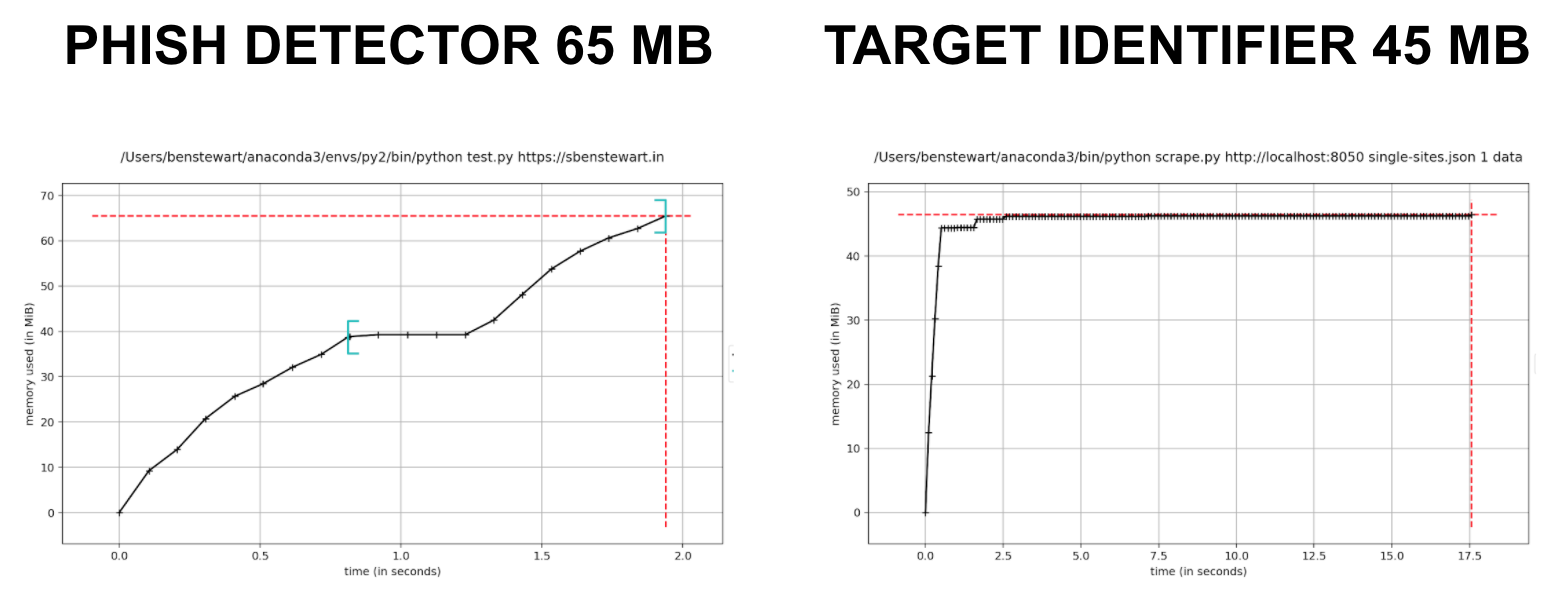
\includegraphics[scale=0.5]{Figures/image15.png}
\caption{Background Process Memory Usage}
\label{fig:bpmu}
\end{figure}

The Figure ~\ref{fig:bpmu} gives the average memory usage for the dispatcher along with the phish detector and the target identifier which in total accounts to 110MB which is the average memory used by an application on 64 bit systems.

\begin{figure}[htp]
\centering
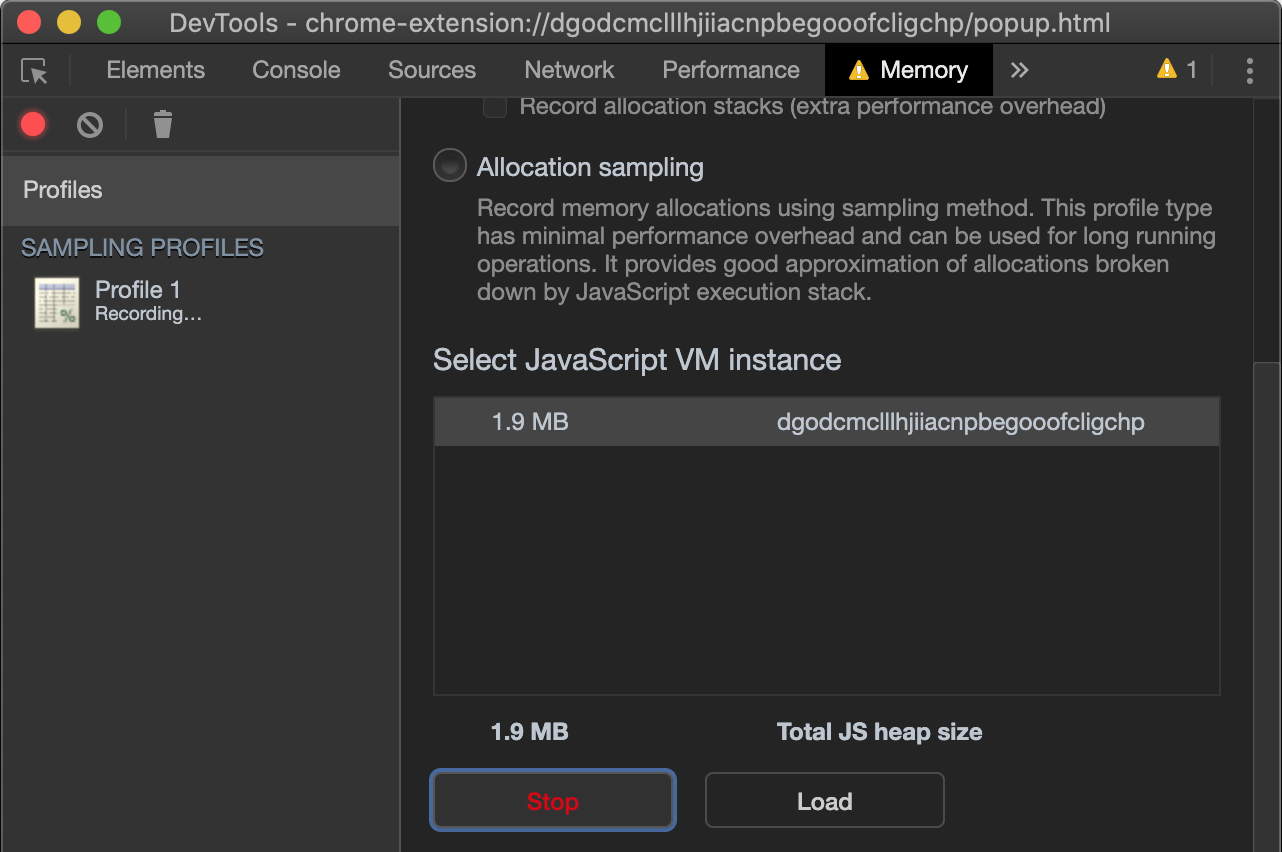
\includegraphics[scale=0.5]{Figures/image6.png}
\caption{Addon Memory Usage}
\label{fig:amu}
\end{figure}

The Figure ~\ref{fig:amu} gives the average memory usage for the add on which includes both the content script and the background script, which is 1.9MB. This is a very reasonable memory requirement for the add-on. Thus in total, the application requires 111.9MB on average.

\section{ADD-ON RENDERING TIME}
Since the add-on has a background component which has to collect the data from multiple tabs that could be running simultaneously, the add-on must be tested to check if it is stable and does not take time to render and thereby blink.\\
\null\quad\textit{Rendering Time = End time - Start time}\\

\begin{figure}[htp]
\centering
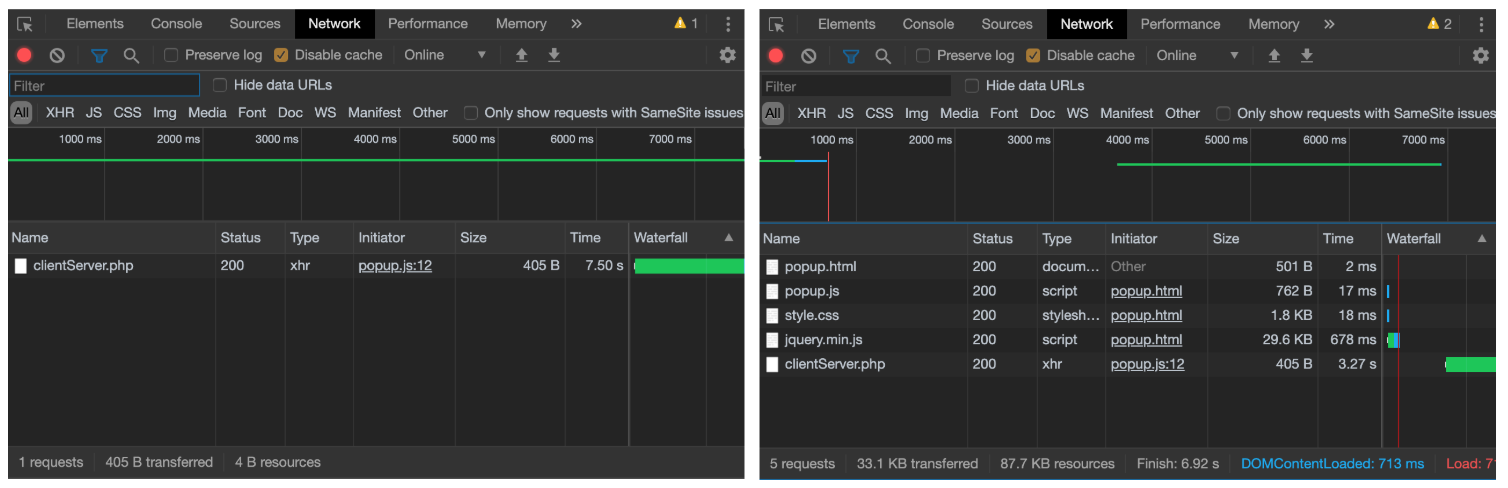
\includegraphics[scale=0.25]{Figures/image14.png}
\caption{Addon Rendering Time}
\label{fig:art}
\end{figure}

The Figure  ~\ref{fig:art} gives the times that it takes for the first time which is 7.5 seconds and for the subsequent times, it drops down to 3.27 seconds which is a bit more than a 50 percent reduction in the execution time. The main reason for this reduction is the auto updated whitelist.

\section{TEMPORAL RESILIENCY ACCURACY}
Temporal resilience accuracy is a metric which says that the application must be resilient to adaptations by the malicious actor, over time. Thus this can be measured by checking if the accuracy does not reduce with the passage of time.\\
\null\quad\textit{Accuracy = (TP+TN)/(TP+TN+FP+FN)}\\

\begin{figure}[htp]
\centering
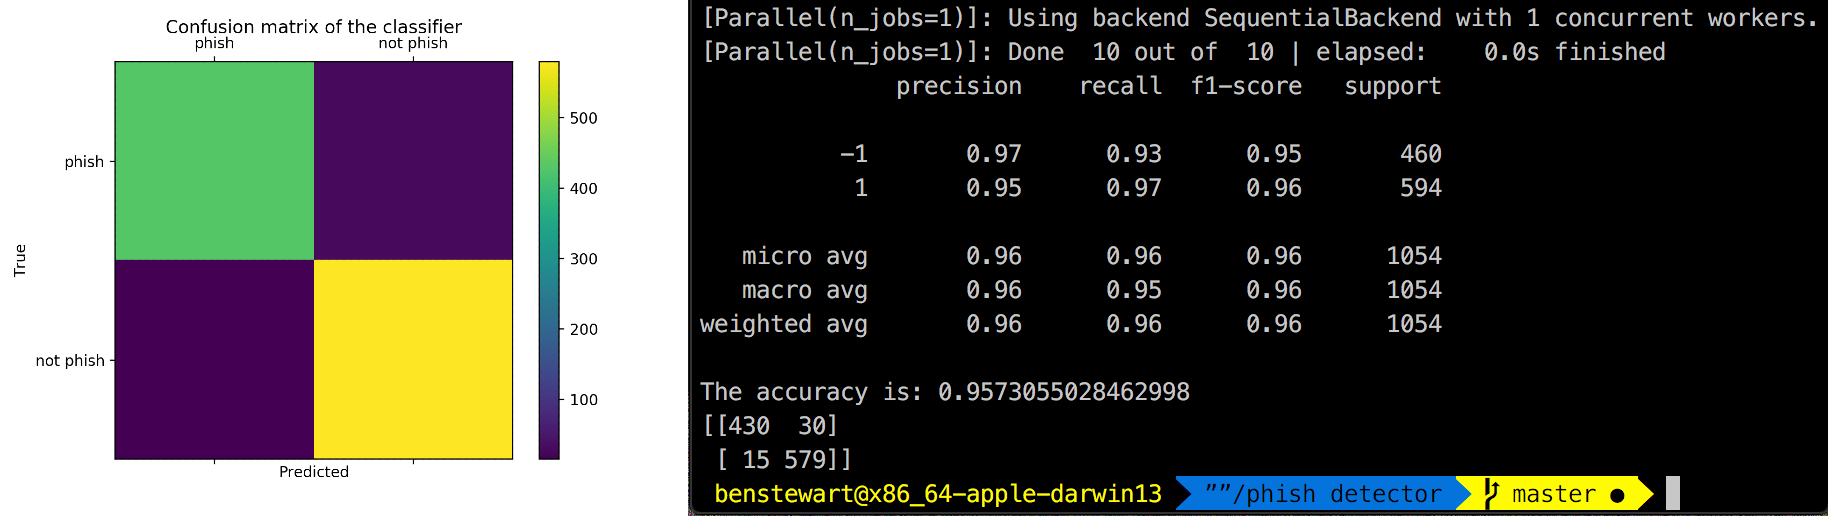
\includegraphics[scale=0.2]{Figures/image8.png}
\caption{Phish Detection Confusion Matrix and Metrics}
\label{fig:pdcmm2}
\end{figure}

The Figure  ~\ref{fig:pdcmm2} gives the phish detection accuracy along with the precision, recall and f1-score for the model run after two months of the first instance being run whose results are in Figure ~\ref{fig:pdcmm}. The accuracy drop from the first run is 0.0035. This makes it almost temporally resilient.

\section{COMPARISONS}
In Table ~\ref{tab:ct2}  we will look into how our system compares with the systems implemented in the previous papers. The metrics that will be compared are the phish detection accuracy, memory usage, execution time and temporal resiliency. The metric of target detection has been omitted because those papers did not implement such a subsystem.

\begin{table}[h!]
\caption{Metrics Comparison Table}
\centering
    \begin{tabular}{ |m{4cm}|m{5cm}|m{5cm}| }
    \hline
    Metric & Previous Benchmark & Off-the-hook-plus \\ \hline
    Phish Detection Accuracy (Percent) & 95.54 & 96.11 \\ \hline
    Memory Usage (MB) & 295 & 111.9 \\ \hline
   Execution Time (seconds) & 8.74 & 7.5 \\ \hline
    Temporal Resiliency (Percent Decrease) & 6.44 & 0.35 \\ \hline
    \end{tabular}
\label{tab:ct2}
\end{table}








